\section{2022春}

\setcounter{yearcounter}{2022}
% \setcounter{page}{1}


\subsection{微分積分}
\prob{%
  次の級数が収束するか、発散するかを判定せよ。
  \begin{gather}
    \sum_{n=0}^{\infty}\frac{(n!)^3}{(3n)!}
  \end{gather}
}
\begin{ans*}
  ${}$
  \dm{a_{n} = \frac{(n!)^3}{(3n)!}}とおくと
  \begin{align}
    \left| \frac{a_{n+1}}{a_{n}} \right|
    &= \frac{\{(n+1)!\}^3}{\{3(n+1)\}!} \tm \frac{(n!)^3}{(3n)!} \\
    &= \frac{(n+1)^3}{(3n+3)(3n+2)(3n+1)} \\
    &= \frac{\biggl(1+\cfrac{1}{n}\biggr)\biggl(1+\cfrac{1}{n}\biggr)}
    {3\biggl(3+\cfrac{2}{n}\biggr)\biggl(3+\cfrac{1}{n}\biggr)} \\
    &\to \frac{1}{27} < 1 \quad(n\to\infty)
  \end{align}
  より収束する。\footnote{appendix}
\end{ans*}


\prob{%
  次の関数$f(x)$が$x=0$において微分可能であるか否かを調べよ。
  ここで、$e$は自然対数の底である。
  \begin{gather}
    f(x) = \frac{x}{1+e^{\frac{1}{x}}}\quad(x\neq 0),\quad f(0) = 0
  \end{gather}
}

\begin{ans*}
  関数$f$についての$x=0$周辺での次の極限を考えるとき
  \begin{align}
    \lim_{\Delta x\to +0}\frac{f(\Delta x) - f(0)}{\Delta x}
    = \lim_{\Delta x\to +0}\frac{1}{1+e^{\frac{1}{x}}}
    = 0 \\
    \lim_{\Delta x\to -0}\frac{f(\Delta x) - f(0)}{\Delta x}
    = \lim_{\Delta x\to -0}\frac{1}{1+e^{\frac{1}{x}}}
    = 1
  \end{align}
  であり、両側極限が一致せず極限が存在しないので微分可能でない。
\end{ans*}


\prob{
  次の重積分について、以下の問いに答えよ。
  \begin{gather}
    \iint_D \sqrt{x^2+y^2}\,dxdy, \quad
    D = \left\{ (x,y) \relmiddle x\geq 0,\, y\geq 0,\, x\leq x^2+y^2\leq 1 \right\}
  \end{gather}
  \begin{enumerate}[label=(\arabic*)]
    \item 積分領域$D$を図示せよ。
    \item この重積分を計算せよ。
  \end{enumerate}
}
\begin{ans*}
  ${}$
  \begin{enumerate}[label=(\arabic*)]
    \item 略 % pic
    \item 極座標変換を考える。
    \begin{align}
      D
      &= \left\{(r,\grt)\relmiddle \cos\grt\geq 0,\, \sin\grt\geq 0,\, r\cos\grt\leq r^2,\, r^2\leq 1\right\} \\
      &= \left\{(r,\grt)\relmiddle 0\leq \grt\leq \frac{\pi}{2},\, r\leq 1,\, \cos\grt \leq r\right\}
    \end{align}
    よって、与えられた積分は
    \begin{align}
      \iint_D \sqrt{x^2+y^2}\,dxdy
      &= \int_{0}^{\pi/2}\int_{\cos\grt}^{1}\, drd\grt [r^2] \\
      &= \int_{0}^{\pi/2}\,d\grt \left[ \frac{1}{3}r^3 \right]_{\cos\grt}^{1} \\
      &= \int_{0}^{\pi/2} \Biggl( \frac{1}{3} - \cos^3\grt \Biggr)\, d\grt \\
      &= \frac{\pi}{6} - \frac{2}{3}
    \end{align}
  \end{enumerate}
\end{ans*}


\prob{%
  次の初期値問題を解け。
  \begin{gather}
    y'' + 2y' + y = 0,\quad y(0) = 1,\quad y'(0) = 0
  \end{gather}
}
\begin{ans*}
  補助方程式$\grl^2+2\grl+1 = (\grl + 1)^2 = 0$より、基本解$y = e^{-x},\,xe^{-x}$の
  線形結合で、任意定数$A,B$を用いて一般解を
  \begin{gather}
    y = (A+Bx)e^{-x}
  \end{gather}
  と得る。
  ここに、初期条件を考慮して$A = 1,\,B = 1$と決定するのでこの解は
  \begin{gather}
    y = (1+x)e^{-x}
  \end{gather}
  である。
\end{ans*}

\newpage
\subsection{線形代数}
\prob{%
  行列$\bA$、ベクトル$\bx,bb$に関する以下の問いに答えよ。
  ここに、
  \begin{gather}
    \bA =
    \pmat{
      -1 & 2 & 1 & -2 \\
      5 & -4 & -1 & 3 \\
      3 & 0 & 2 & 3 \\
      2 & -4 & 2 & 3
    }
    ,\quad
    \bx =
    \pmat{
      x_1 \\ x_2 \\ x_3 \\ x_4
    }
    ,\quad \bb =
    \pmat{
      3 \\ -2 \\ c \\ 0
    }
  \end{gather}
  であり、$x_i\:(i = 1,\cdots ,\,4)$および$c$は実数である。
  \begin{enumerate}[label=(\arabic*)]
    \item $\rank\bA$を求めよ。
    \item $\bA$の行列式を求めよ。
    \item 連立方程式$\bA\bx = \bb$が解を持たないときの$c$を求めよ。
  \end{enumerate}
}
\begin{ans*}
  ${}$
  \begin{enumerate}[label=(\arabic*)]
    \item
    \begin{align}
      \bA
      &\lra
      \bmat{
        1 & -2 & -1 & 2 \\
        0 & 6 & 4 & -7 \\
        0 & 6 & 4 & -7 \\
        0 & 0 & 4 & -1
      } \\
      &\lra
      \bmat{
        1 & -2 & -1 & 2 \\
        0 & 6 & 4 & -7 \\
        0 & 0 & 4 & 1 \\
        0 & 0 & 0 & 0
      }
    \end{align}
    より$\rank\bA = 3$

    \item
    \begin{gather}
      \det\bA
      = 3\det\bmat{
        2 & 1 & -2 \\
        -4 & -1 & 3 \\
        -4 & 2 & 3
      } + \det \bmat{
        -1 & 2 & -2 \\
        5 & -4 & 3 \\
        2 & -4 & 3
      } + \det \bmat{
        -1 & 2 & 1 \\
        5 & -4 & -1 \\
        2 & -4 & 2
      } \\
      = 18 + 6 - 24 = 0
    \end{gather}
    \item $\bA\bx = \bb$が解を持たないことの必要十分条件は$\rank\bA \neq \rank(\bA|\bb)$である。
    \begin{align}
      [\bA|\bb]
      &\lra \left[\begin{array}{cccc|c}
        -1 & 2 & 1 & -2 & 3 \\
        5 & -4 & -1 & 3 & 2 \\
        3 & 0 & 1 & -1 & c \\
        2 & -4 & 2 & 3 & 0
      \end{array}\right] \\
      &\lra \left[\begin{array}{cccc|c}
        1 & -2 & -1 & 2 & 3 \\
        0 & 6 & 4 & -7 & 13 \\
        0 & 6 & 4 & -7 & c+9\\
        0 & 0 & 4 & -1 & 6
      \end{array}\right] \\
      &\lra\left[\begin{array}{cccc|c}
        1 & -2 & -1 & 2 & 3  \\
        0 & 6 & 4 & -7 & 13 \\
        0 & 0 & 4 & 1 & 6 \\
        0 & 0 & 0 & 0 & c-4
      \end{array}\right]
    \end{align}
    ゆえに
    \begin{gather}
      \rank(\bA|\bb) =
      \begin{dcases*}
        3 & (c = 4) \\
        4 & (c \neq 4)
      \end{dcases*}
    \end{gather}
    よって、$\bA\bx = \bb$が解を持たないような$c$は$c\neq 4$である。
  \end{enumerate}
\end{ans*}


\prob{%
  次の2次形式について以下の問いに答えよ。
  \begin{gather}
    f(x,y,z) = \frac{1}{16}\bigl(13x^2 + 6\sqrt{3}xy + 7y^2 + 16z^2\bigr)
  \end{gather}
  \begin{enumerate}[label=(\arabic*)]
    \item $f(x,y,z)$の標準形を求めよ。
    \item $f(x,y,0)=1$の概形を描け。
  \end{enumerate}
}

\begin{ans*}
  ${}$
  \begin{enumerate}[label=(\arabic*)]
    \item 標準形$\bx^{\top} \bA \bx (=\ip{\bx,\bA\bx})$に直す。
    \begin{gather}
      f(x,y,z)
      = \frac{1}{16}
      \Bmat{x & y & z}
      \bmat{
        13 & 3\sqrt{3} & 0 \\
        3\sqrt{3} & 7 & 0 \\
        0 & 0 & 16
      }\Bmat{
        x \\ y \\ z
      }
    \end{gather}

    \item $f(x,y,0) = 1$は
    \begin{gather}
      \Bmat{x & y}\frac{1}{16}
      \bmat{
        13 & 3\sqrt{3} \\
        3\sqrt{3} & 7
      }\Bmat{
        x \\ y
      } = 1
    \end{gather}
    と変形できる。このとき、行列をあらたに
    \begin{gather}
      \bB =\frac{1}{16}\bmat{
        13 & 3\sqrt{3} \\
        3\sqrt{3} & 7
      }
    \end{gather}
    とおく。このとき、$\bB$の固有値は補助方程式
    \begin{align}
      \det(\bA - \grl\bE) = (\grl - 1)\biggl(\grl - \frac{1}{4}\biggr) = 0
    \end{align}
    より、\dm{\grl = 1, \frac{1}{4}\:(=:\grl_1,\, \grl_2)}である。
    \begin{enumerate}[label=(\roman*)]
      \item $\grl = \grl_1$のとき、固有ベクトル\dm{\bu_1 = \Bmat{u \\v}}は
      \begin{gather}
        \bmat{
          \disp -\frac{3}{16} & \disp \frac{3\sqrt{3}}{16} \\
          & \\
          \disp \frac{3\sqrt{3}}{16} & \disp-\frac{9}{16}
        }\Bmat{\disp u \\ \\ \disp v} = \bzv \\
        \therefore \bu_1 = \Bmat{
          \disp \frac{\sqrt{3}}{2} \\
          \\
          \disp \frac{1}{2}
        }
      \end{gather}
      \item $\grl = \grl_2$のとき、固有ベクトル$\bu_2$は
      \begin{gather}
        \bmat{
          \disp \frac{9}{16} & \disp \frac{3\sqrt{3}}{16} \\
          & \\
          \disp \frac{3\sqrt{3}}{16} & \disp\frac{3}{16}
        }\Bmat{u  \\ \\ v} = \bzv \\
        \therefore \bu_2 = \Bmat{
          \disp -\frac{1}{2} \\
          \\
          \disp \frac{\sqrt{3}}{2}
        }
      \end{gather}
    \end{enumerate}
    ここでこれらの固有ベクトルを横に並べた行列$\bP := [\bu_1 ,\, \bu_2]$を考える。
    この行列は
    \begin{gather}
      \bP
      =
      \bmat{
          \disp \frac{\sqrt{3}}{2} & \disp -\frac{1}{2} \\
          \\
          \disp \frac{1}{2} & \disp \frac{\sqrt{3}}{2}
      } =
      \bmat{
        \disp \cos\frac{\pi}{6} &\disp \sin\frac{\pi}{6} \\
        & \\
        \disp -\sin\frac{\pi}{6} &\disp \cos\frac{\pi}{6} \\
      }
    \end{gather}
    であるので、\dm{\frac{\pi}{6}}方向の回転行列である。
    \dm{\Bmat{X \\ Y} = \bP\Bmat{x \\y}}の座標変換によって
    \begin{align}
      &f(x, y, 0) = 1 \\
      &\quad\eqa
      \Bmat{x & y}\bP^{-1}\bP\bA\bP^{-1}\bP\Bmat{x \\ y} \\
      &\quad\eqa
      \Bmat{X & Y}\bP\bA\bP^{-1}\Bmat{X \\ Y} \\
      &\quad\eqa
      \Bmat{X & Y}\bmat{1 & 0 \\ 0 & 1/4}\Bmat{X \\ Y} \\
      &\quad\eqa
      X^2 + \frac{Y^2}{4} = 1
    \end{align}
    に移るので楕円を表す。

    \begin{figure}[H]\centering
      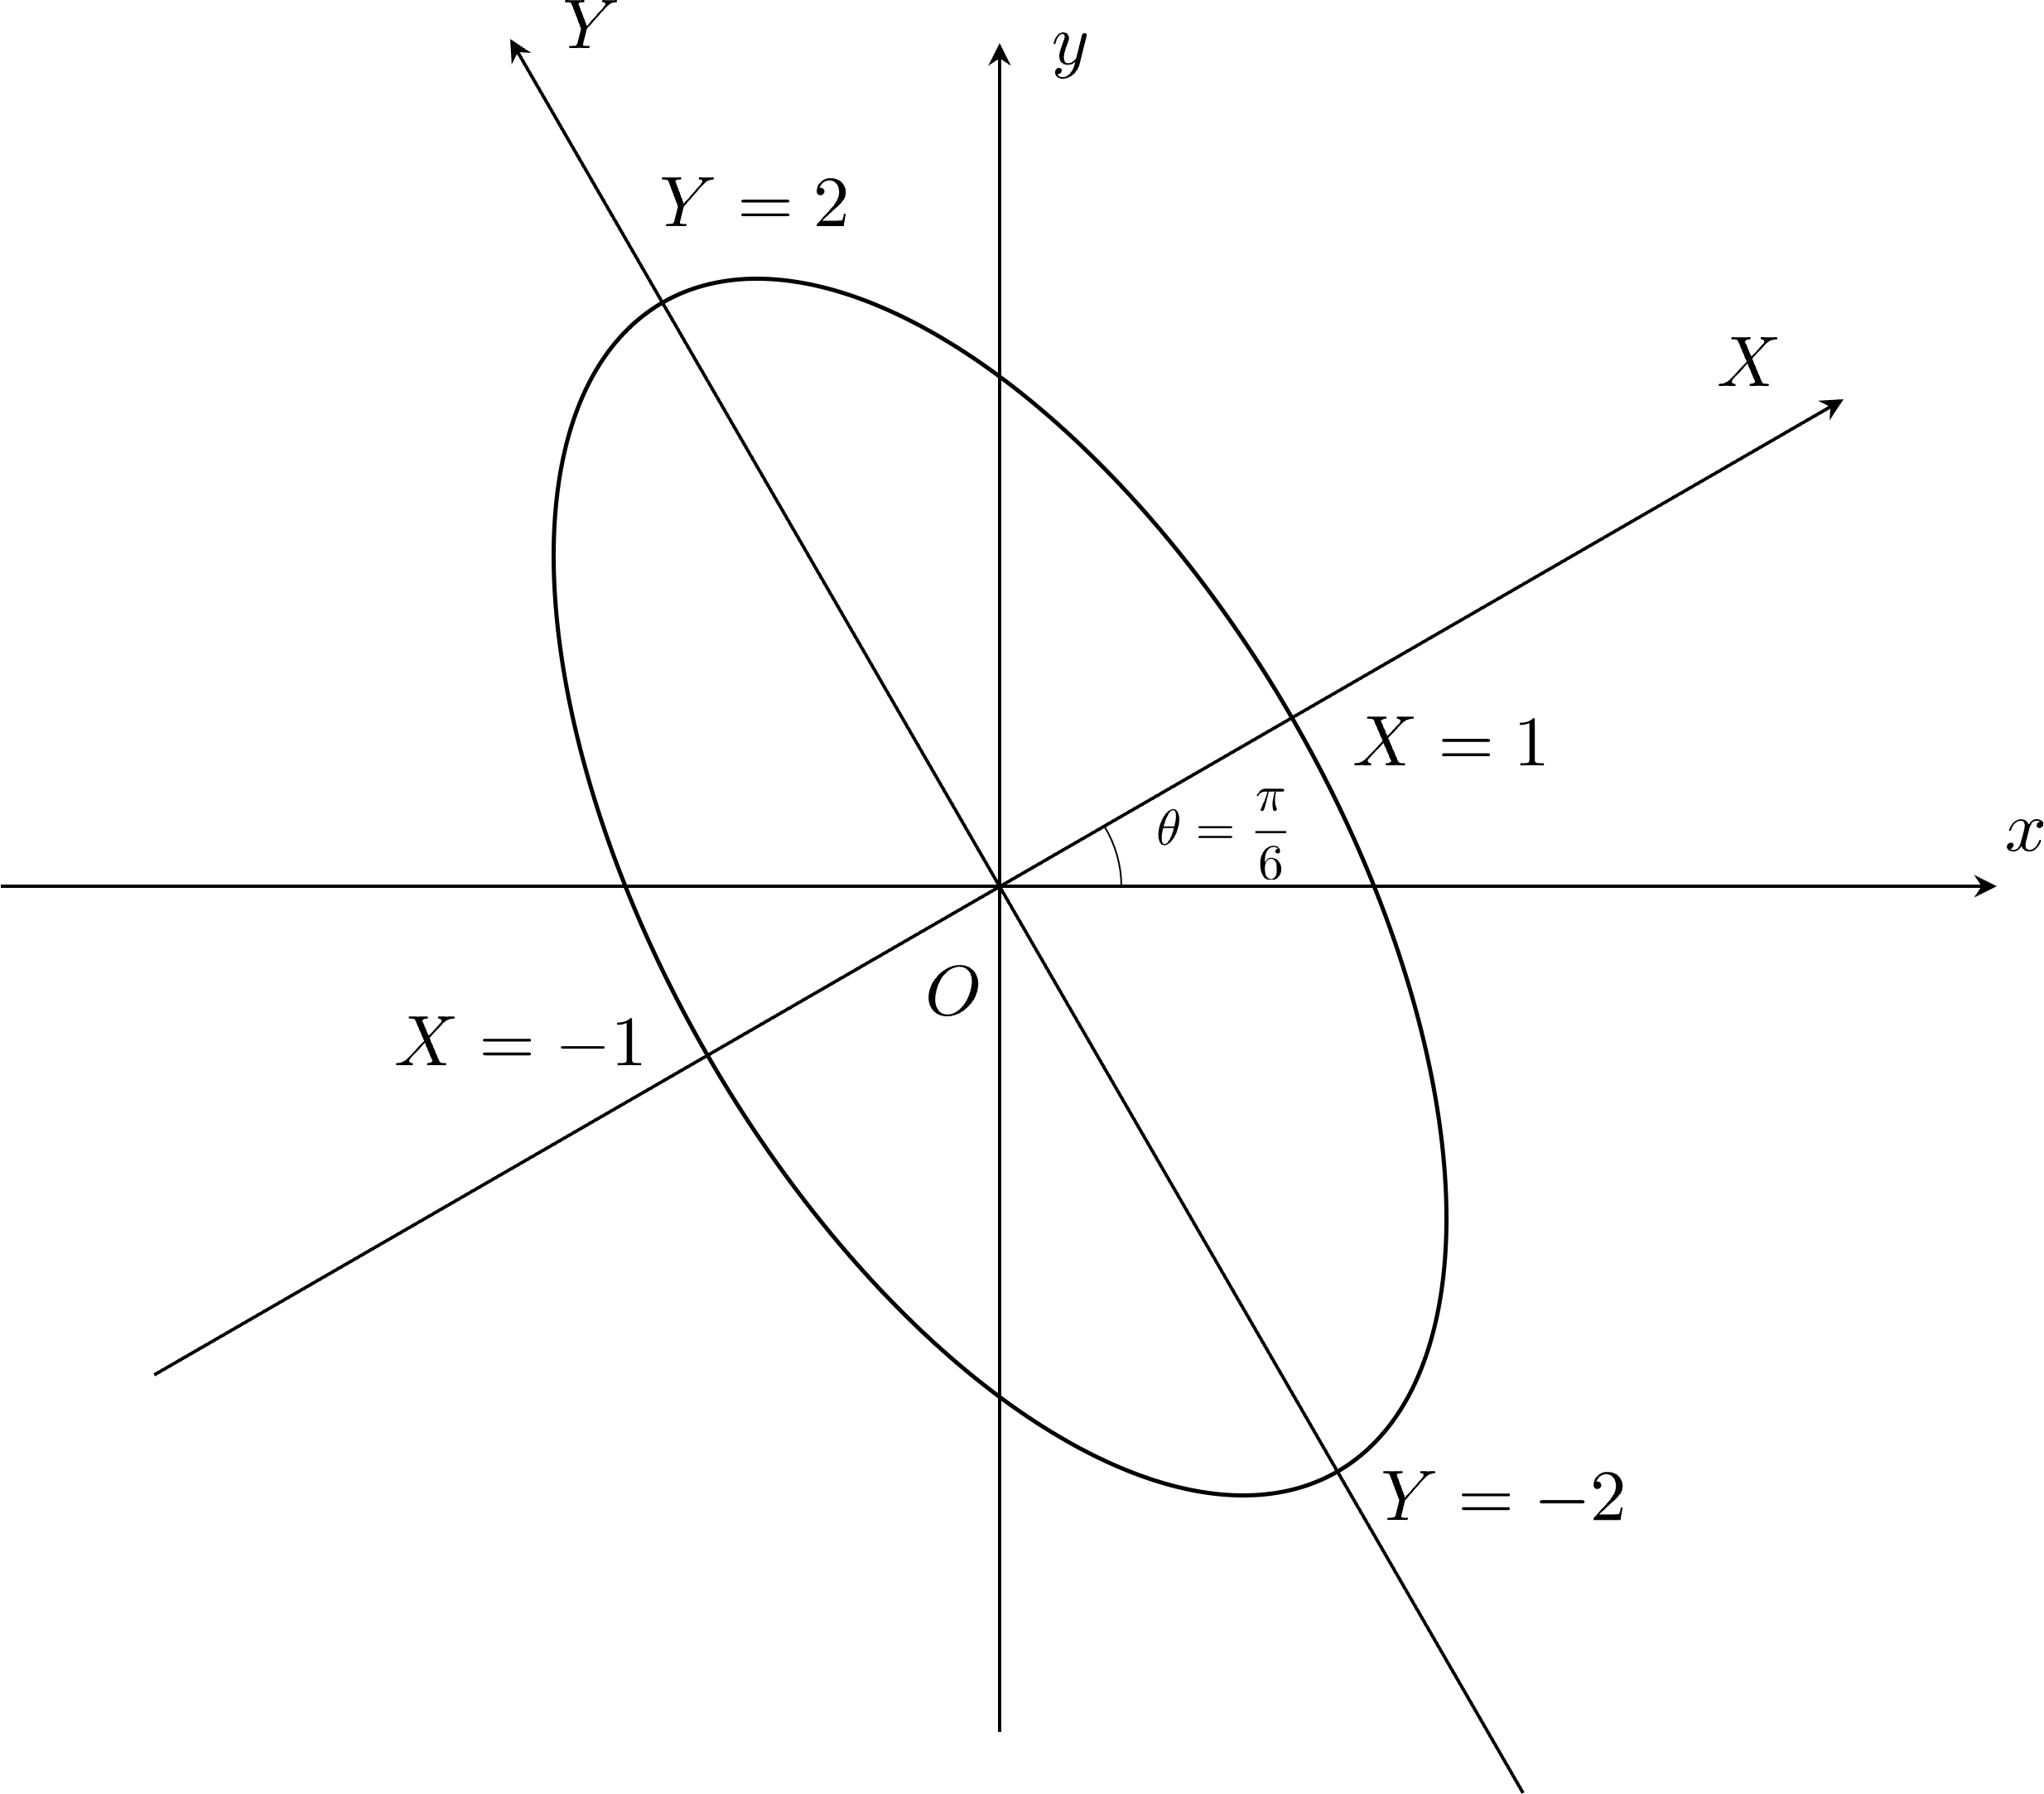
\includegraphics[width=.6\linewidth]{./src/fig/Basic/B_2020_spring_fxy0.png}
    \end{figure}

  \end{enumerate}
\end{ans*}
